%%%%%%%%%%%%%%%%%%%%%%%%%%%%%%%%%%%%%%%%%
% Beamer Presentation
% LaTeX Template
% Version 1.0 (10/11/12)
%
% This template has been downloaded from:
% http://www.LaTeXTemplates.com
%
% License:
% CC BY-NC-SA 3.0 (http://creativecommons.org/licenses/by-nc-sa/3.0/)
%
%%%%%%%%%%%%%%%%%%%%%%%%%%%%%%%%%%%%%%%%%

%----------------------------------------------------------------------------------------
%   PACKAGES AND THEMES
%----------------------------------------------------------------------------------------

\documentclass{beamer}

\mode<presentation> {

% The Beamer class comes with a number of default slide themes
% which change the colors and layouts of slides. Below this is a list
% of all the themes, uncomment each in turn to see what they look like.

%\usetheme{default}
%\usetheme{AnnArbor}
%\usetheme{Antibes}
%\usetheme{Bergen}
%\usetheme{Berkeley}
%\usetheme{Berlin}
%\usetheme{Boadilla}
%\usetheme{CambridgeUS}
%\usetheme{Copenhagen}
%\usetheme{Darmstadt}
%\usetheme{Dresden}
%\usetheme{Frankfurt}
%\usetheme{Goettingen}
%\usetheme{Hannover}
%\usetheme{Ilmenau}
%\usetheme{JuanLesPins}
%\usetheme{Luebeck}
\usetheme{Madrid}
%\usetheme{Malmoe}
%\usetheme{Marburg}
%\usetheme{Montpellier}
%\usetheme{PaloAlto}
%\usetheme{Pittsburgh}
%\usetheme{Rochester}
%\usetheme{Singapore}
%\usetheme{Szeged}
%\usetheme{Warsaw}

% As well as themes, the Beamer class has a number of color themes
% for any slide theme. Uncomment each of these in turn to see how it
% changes the colors of your current slide theme.

%\usecolortheme{albatross}
%\usecolortheme{beaver}
%\usecolortheme{beetle}
%\usecolortheme{crane}
%\usecolortheme{dolphin}
%\usecolortheme{dove}
%\usecolortheme{fly}
%\usecolortheme{lily}
%\usecolortheme{orchid}
%\usecolortheme{rose}
%\usecolortheme{seagull}
%\usecolortheme{seahorse}
%\usecolortheme{whale}
%\usecolortheme{wolverine}

%\setbeamertemplate{footline} % To remove the footer line in all slides uncomment this line
%\setbeamertemplate{footline}[page number] % To replace the footer line in all slides with a simple slide count uncomment this line

%\setbeamertemplate{navigation symbols}{} % To remove the navigation symbols from the bottom of all slides uncomment this line
}

\usepackage{graphicx} % Allows including images
\usepackage{booktabs} % Allows the use of \toprule, \midrule and \bottomrule in tables
\usepackage[utf8]{inputenc}
\usepackage[czech]{babel}

%----------------------------------------------------------------------------------------
%   TITLE PAGE
%----------------------------------------------------------------------------------------



\title[Masarykova univerzita]{Rozšíření možností zaznamenávání událostí v aplikačním serveru WildFly} % The short title appears at the bottom of every slide, the full title is only on the title page

\author{Radek Koubský} % Your name
\institute[Fakulta informatiky] % Your institution as it will appear on the bottom of every slide, may be shorthand to save space
{
Masarykova univerzita \\ % Your institution for the title page
\medskip
\textit{Fakulta informatiky} % Your email address
}
\date{19. února 2016} % Date, can be changed to a custom date

\begin{document}

\begin{frame}
\titlepage % Print the title page as the first slide
\end{frame}

\begin{frame}
\frametitle{Osnova} % Table of contents slide, comment this block out to remove it
\tableofcontents % Throughout your presentation, if you choose to use \section{} and \subsection{} commands, these will automatically be printed on this slide as an overview of your presentation
\end{frame}

%----------------------------------------------------------------------------------------
%   PRESENTATION SLIDES
%----------------------------------------------------------------------------------------

\begin{frame}
	\frametitle{Motivace}
	\begin{itemize}
		\item zpracování velkého množství logovacích záznamů
		\begin{itemize}
			\item cloudové prostředí
			\item více instancí serveru
		\end{itemize}
		\item vizualizace a analýza logovacích záznamů
		\item nedostatek logovací informace
		\item přidání nové logovací informace bez modifikace zdrojového kódu
	\end{itemize}
\end{frame}

%------------------------------------------------
\section{Klíčové technologie} % Sections can be created in order to organize your presentation into discrete blocks, all sections and subsections are automatically printed in the table of contents as an overview of the talk
%------------------------------------------------

\subsection{WildFly}
\begin{frame}
	\frametitle{Aplikační server WildFly (JBoss)}
	\begin{itemize}
		\item úplná implementace Java EE 7
		\item architektura: jádro + podsystémy
		\item JBoss Modules nahrávání tříd
		\item Open Source - JBoss Community
		\item dynamický vývoj (aktuální verze 10)
	\end{itemize}
\end{frame}

\subsection{Elasticsearch \& Kibana} % A subsection can be created just before a set of slides with a common theme to further break down your presentation into chunks

\begin{frame}
\frametitle{Elasticsearch \& Kibana}
\begin{itemize}
	\item Elasticsearch
	\begin{itemize}
		\item distribuovaný úložný systém
		\item indexace každého pole (data ve formátu JSON)
		\item real-time analýza dat
		\item výkonný vyhledávací engine postavený na Apache Lucene
		\item vysoká škálovatelnost
		\item RESTFul, Java API
	\end{itemize}
	\item Kibana
	\begin{itemize}
		\item vyhledávání, vizualizace a analýza dat v Elasticsearch
	\end{itemize}
\end{itemize}
\end{frame}

%------------------------------------------------
\subsection{Byteman}
\begin{frame}
	\frametitle{(\textbf{Byte})code (\textbf{Man})ipulation}
\begin{itemize}
	\item Byteman Rule engine, Byteman Rules
	\item Event Condition Action pravidla
	\begin{enumerate}
		\item pokud nastane \textit{Událost}
		\item a \textit{Podmínka} je splněna
		\item vykonej \textit{Akci}
	\end{enumerate}
	\item Rule Helper
	\item Java agent
	\item Byteman vs. AspectJ
\end{itemize}
\end{frame}

%------------------------------------------------
\section{Rozšíření zaznamenávání událostí ve WildFly}
%------------------------------------------------

\begin{frame}
	\frametitle{Požadavky na rozšíření}
	
	\begin{itemize}
		\item ukládání událostí do Elaticsearch
		\item vizualizace událostí pomocí nástroje Kibana
		\item přidání nových událostí do vybraných částí WildFly
		\begin{itemize}
			\item \textit{Web Container (Servlets, JSPs)}
			\item \textit{REST endpoints}
			\item \textit{WS endpoints}
			\item \textit{EJB invocations}
			\item \textit{JMS communication}
		\end{itemize}
		\item přidání nových událostí bez modifikace zdrojového kódu Wildfly
	\end{itemize}
\end{frame}

\begin{frame}
\frametitle{Architektura rozšíření}
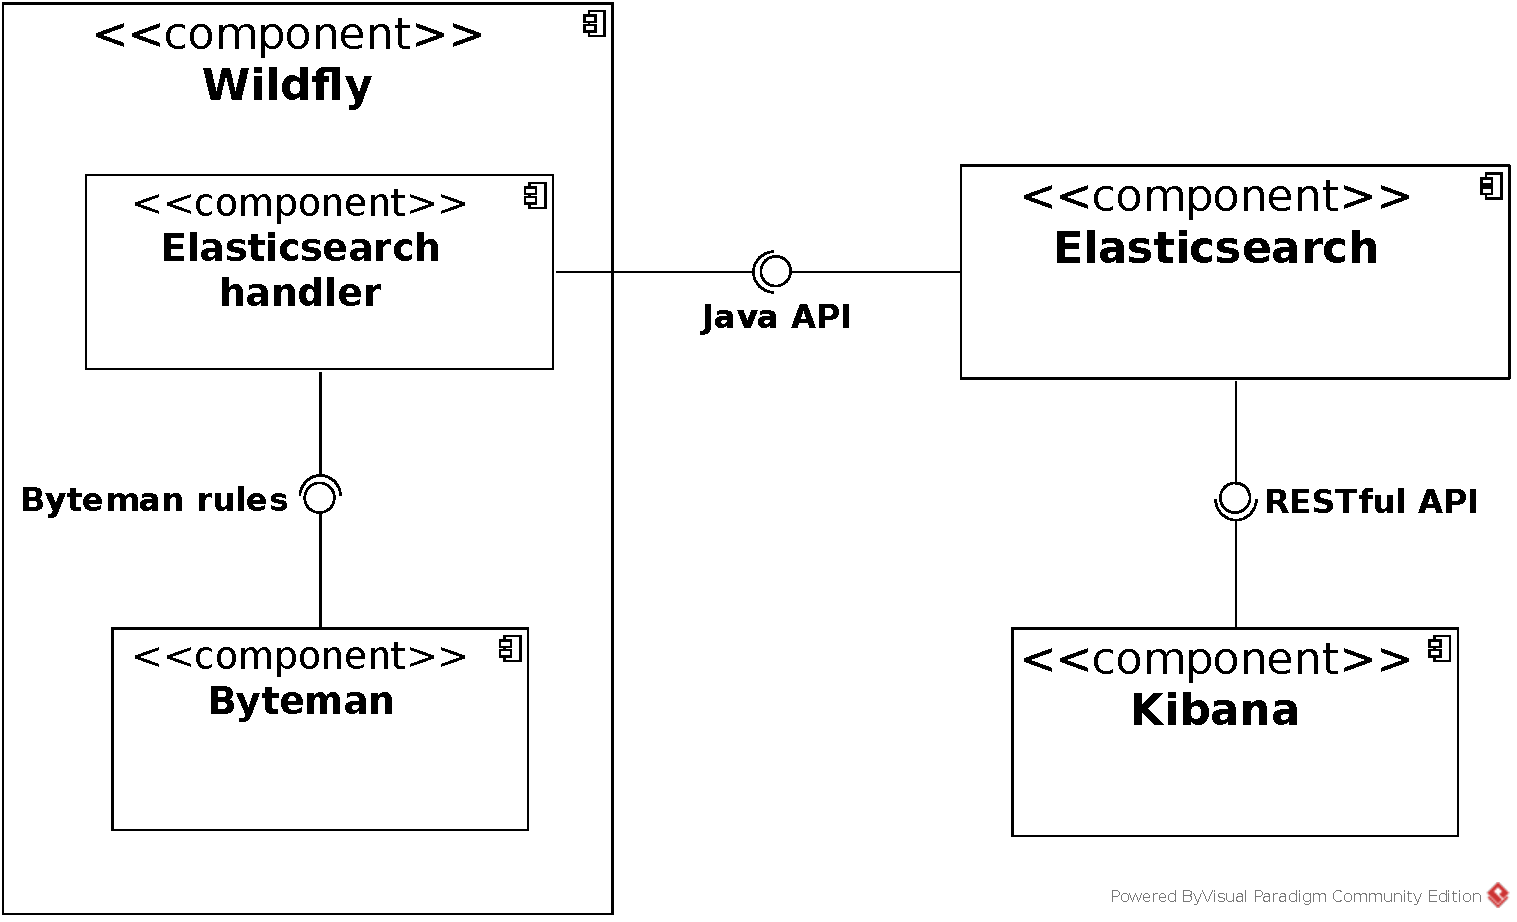
\includegraphics[width=\textwidth]{../images/component_diagram}
\end{frame}

%------------------------------------------------

\subsection{elasticsearch-wildfly-log}

\begin{frame}
	\frametitle{elasticsearch-wildly-log}
	\begin{itemize}
		\item rozšíření logovacího podsystému Wildfly
		\begin{itemize}
			\item Custom Log Handler
		\end{itemize}
		\item připojení k Elasticsearch
		\item převod události do formátu JSON
		\item přidání jména a adresy serveru k události
		\item uložení události do Elasticsearch
	\end{itemize}
\end{frame}

\begin{frame}
\frametitle{Vizualizace událostí v nástroji Kibana}
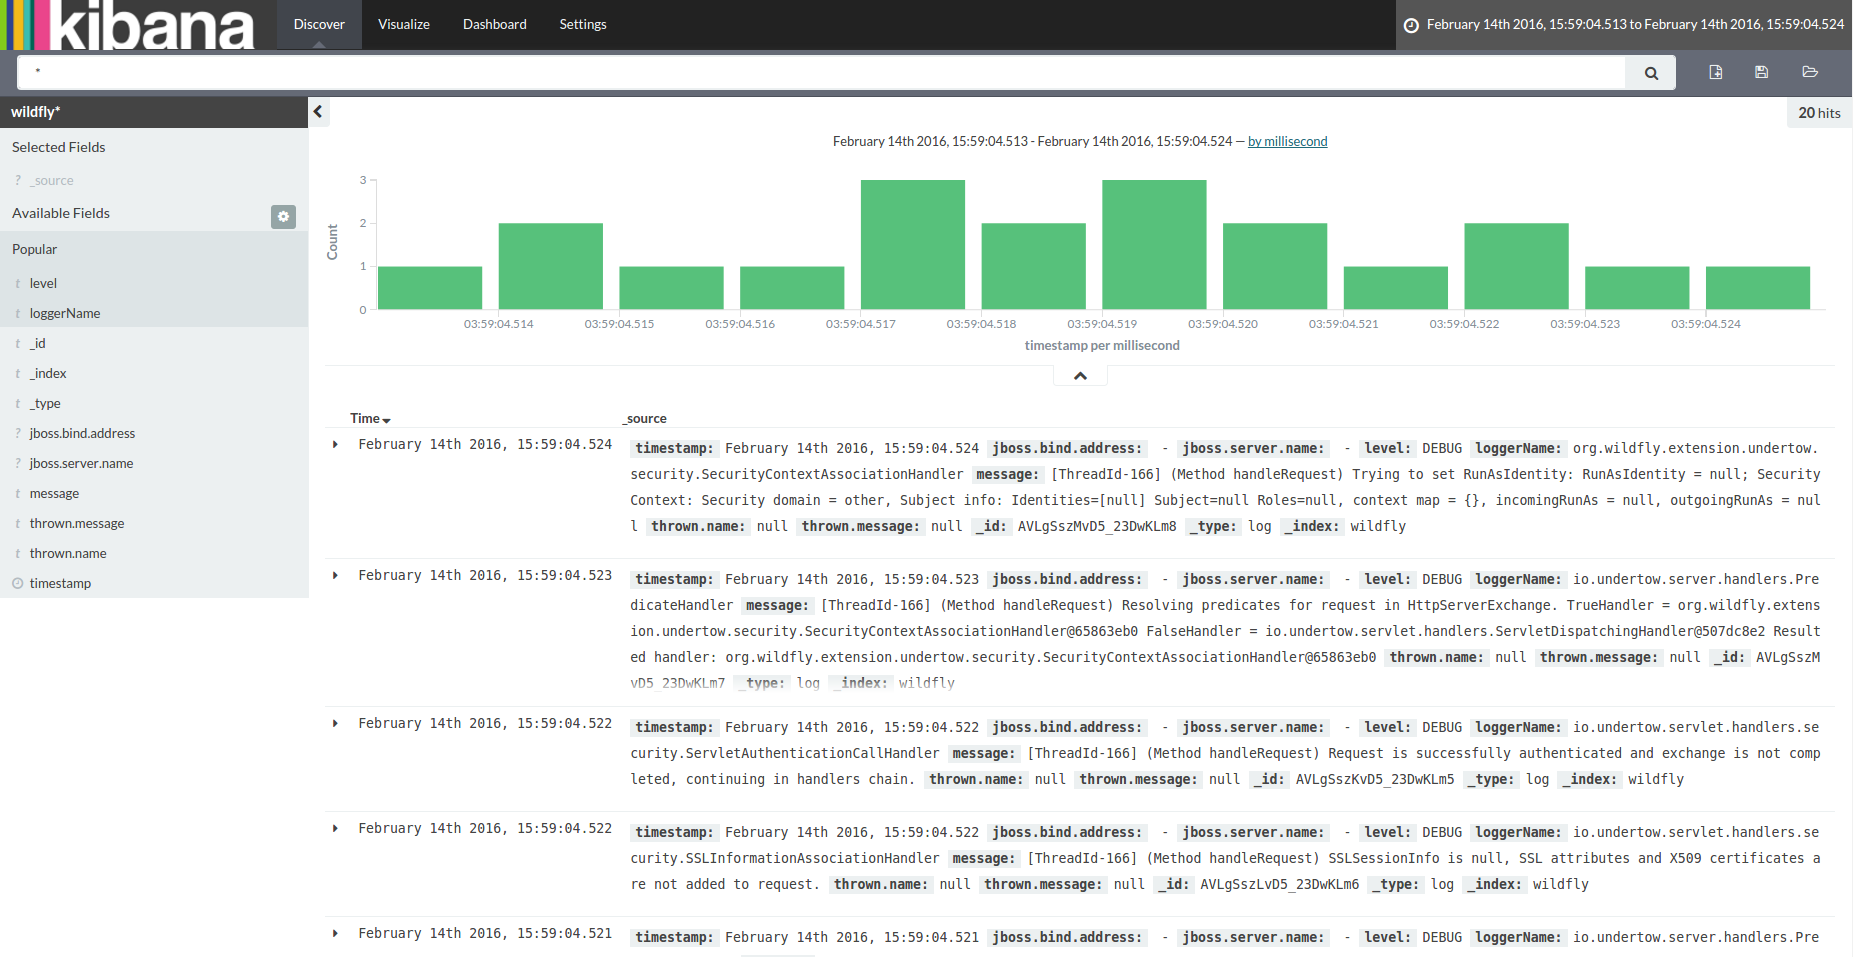
\includegraphics[width=\textwidth]{kibana}
\end{frame}

%------------------------------------------------
\subsection{byteman-wildfly-log}
\begin{frame}[fragile] % Need to use the fragile option when verbatim is used in the slide
\frametitle{byteman-wildfly-log}
\begin{itemize}
	\item vkládání nových logovacích záznamů do vybraných částí serveru pomocí pravidel Byteman
	\begin{itemize}
		\item \textit{Web Container (Servlets, JSPs)}
		\item \textit{REST endpoints}
		\item \textit{WS endpoints}
		\item \textit{EJB invocations}
		\item \textit{JMS communication}
	\end{itemize}
	\item celkem přidáno 226 logovacích událostí
	\item Log Helper
	\item přidávání globálních informací do logovacích záznamů (thread-id)
\end{itemize}
\end{frame}

%------------------------------------------------

\section{Shrnutí}
\subsection{Přínos, problémy, práce do budoucna}
\begin{frame}
	\frametitle{Problémy během implementace}
	\begin{itemize}
		\item BYTEMAN-298, BYTEMAN-299
		\begin{itemize}
			\item vydána verze Byteman 3.0.2 (Byteman blog)
		\end{itemize}
		\item konflikt mezi Byteman a JBoss Modules (16. 7. 2015)
		\begin{itemize}
			\item návrh řešení (Andrew Dinn)
			\item dokončení experimentální implementace (JBoss Modules plugin)
			\item vydáno ve verzi Byteman 3.0.2 (24. 11. 2015)
		\end{itemize}
	\end{itemize}
\end{frame}

\begin{frame}
	\frametitle{Přínos}
	\begin{itemize}
		\item centralizovaná správa logovacích záznamů
		\item nástroj pro monitorování/debugging serveru
		\begin{itemize}
			\item možnost přidání/odebraní logovací informace na libovolné místo v serveru
			\item nezávislé na konkrétní verzi WildFly
			\item princip agenta lze aplikovat na jakýkoliv jiný aplikační server
		\end{itemize}
		\item rozšíření Open Source projektu Byteman
		\item oba projekty zdokumentovány a umístěny na GitHub
	\end{itemize}
\end{frame}

\begin{frame}
	\frametitle{Práce do budoucna}
	\begin{itemize}
		\item testování výkonosti pro další optimalizace
		\begin{itemize}
			\item výkon Byteman rozšíření
			\item výkon Elasticsearch rozšíření
		\end{itemize}
	\end{itemize}
	
\end{frame}

%----------------------------------------------------------------------------------------

\end{document}